
\documentclass[11pt,a4paper]{article}
\author{TalentSprint}
\date{}
\usepackage{verbatim}
\usepackage{fancyhdr}           % For header and footer
\usepackage{multicol}
\usepackage{colortbl}           % For coloured tables
\usepackage{setspace}           % For line height
\usepackage{seqsplit}           % Splits long words.
\usepackage{amsmath} 
\usepackage{graphicx}
\usepackage{array}
\usepackage{enumitem}
\usepackage{xcolor}
\usepackage[tikz]{bclogo}
\usepackage{textcomp}
\usepackage{listings}
\lstset{language=python,numbers=left,numberstyle=\tiny,numbersep=10pt,showstringspaces=false}

\headheight=14pt
\lhead{\nouppercase{}}
\rhead{\nouppercase{\leftmark}}

\newcommand*\lstinputpath[1]{\lstset{inputpath=#1}}
\lstinputpath{../Code}
\graphicspath{{../Images/} {../ScreenShots/}}

\setcounter{tocdepth}{1}
\setlength\parindent{0pt}
\parskip=4pt
\newcommand{\Code}[1]{\textbf{\texttt{#1}}}

% Lengths and widths
\addtolength{\textwidth}{5cm}
\addtolength{\hoffset}{-1cm}
\setlength{\headsep}{-12pt} % Reduce space between header and content
\setlength{\headheight}{85pt} % If less, LaTeX automatically increases it
\renewcommand{\footrulewidth}{2pt} % Remove footer line
\renewcommand{\headrulewidth}{1pt} % Remove header line
\renewcommand{\seqinsert}{\ifmmode\allowbreak\else\-\fi} % Hyphens in seqsplit
% This two commands together give roughly
% the right line height in the tables
\renewcommand{\arraystretch}{1.3}
\onehalfspacing

% Commands
\newcommand{\SetRowColor}[1]{\noalign{\gdef\RowColorName{#1}}\rowcolor{\RowColorName}} % Shortcut for row colour
\newcommand{\mymulticolumn}[3]{\multicolumn{#1}{>{\columncolor{white}}#2}{#3}} % For coloured multi-cols
\newcolumntype{x}[1]{>{\raggedright}p{#1}} % New column types for ragged-right paragraph columns
\newcommand{\tn}{\tabularnewline} % Required as custom column type in use

% Font and Colours
\definecolor{HeadBackground}{HTML}{333333}
\definecolor{FootBackground}{HTML}{666666}
\definecolor{TextColor}{HTML}{333333}
\definecolor{DarkBackground}{HTML}{6B8E23} %{FD1AA8}
\definecolor{LightBackground}{HTML}{E8FED8} %D3FDC8
\definecolor{tit}{HTML}{FF6600}
\renewcommand{\familydefault}{\sfdefault}
\color{TextColor}
 \headsep = 25pt
% Header and Footer
\pagestyle{fancy}
\usepackage[headheight=110pt]{geometry}
\fancyhf{}% Clear header/footer

\fancyhead[r]{
\includegraphics[width = 4cm, height = 2cm]{TS-Logo.png}\hspace{0cm}}

%=================================TITLE=====================================
\fancyhead[l]{\Large{\bf{\textcolor{tit}{\textrm{Arrays}}}}}
%===========================================================================

\renewcommand{\headrulewidth}{0.4pt}% Default \headrulewidth is 0.4pt
\renewcommand{\footrulewidth}{0.4pt}% Default \footrulewidth is 0pt

\rfoot{Page \thepage}
\lfoot{COPYRIGHT \textcopyright TALENTSPRINT, 2015. ALL RIGHTS RESERVED.}




\begin{document}

%\chapter{Arrays and Pointers}
In C programming, one of the frequent problems is to handle similar types of data. For example, the user want to store marks of 100 students. We can do this by creating 100 variables individually.  But this is tedious and impractical and error-prone. Arrays are intended for such uses.

\section*{Array}
Array is a collection of \emph{homogenous} data stored under one name. The values in an array are called as `elements' of an array. These elements are accessed by numbers called as `subscripts' or `indices'. The index of the first element of an array is 0.

\subsection*{Types of Arrays}
Arrays are of two types:
\begin{enumerate}
\item One dimensional arrays
\item Multi-dimensional arrays
\end{enumerate}

\subsection*{One dimensional arrays} 
The array which is used to represent and store data in a linear form is called as `single' or one dimensional array.
\subsubsection*{Declaration} 
Arrays must be declared before they can be used in the program. Standard array declaration is as follows:

\textbf{\texttt{data\_type array\_name[size];}}

Here \texttt{size} is the number of elements that you plan to store in the array.

\lstinline!int halley[5];! 

Here, the name of array is halley. The size of array is 5; there are 5 items (elements) of array halley. The first element is halley[0] and the last is halley[4].


\begin{table}[ht]
\centering
\begin{tabular}{|c|c|c|c|c|}
halley[0]& halley[1]& halley[2]& halley[3]& halley[4]\\\hline
& & & & \\\hline
\end{tabular}
\caption{Uninitialized array}
\label{UninitializedArray}
\end{table}


You must follow these rules when you declare an array in C:
\begin{itemize}
\item The data type can be any valid data type  such as \lstinline!int, float, char,  struct!  or  \lstinline!union!.
\item The name of an array must follow  naming  rules of variables.
\item The size of the array must be a constant positive integer. 
\end{itemize}

\subsection*{Initialization}
 Arrays can be initialized at declaration time. 

\lstinline!int halley[5] = {2061, 1986, 1910, 1835, 1759};!

It is not necessary to define the size of arrays during initialization, \emph{if all the elements you need are being initialized}

\lstinline!int halley[ ] = {2061, 1986, 1910, 1835, 1759};!

In this case, the compiler determines the size of array by calculating the number of elements of an array.

\begin{table}[ht]
\centering
\begin{tabular}{|c|c|c|c|c|}
halley[0]& halley[1]& halley[2]& halley[3]& halley[4]\\\hline
2221 & 2242 & 2234 & 2223 & 2254\\\hline
\end{tabular}
\caption{Initialized array}
\label{InitializedArray}
\end{table}

\subsection*{Accessing array elements}

Arrays can be accessed and treated like variables in  C. For example,

\begin{lstlisting}
    scanf(``%d'', &halley[2]);
    /* --------------------------------------- *
     * statement to insert value in the third  *
     * element of array halley.                 *
     * --------------------------------------- */

    scanf(``%d'', &halley[i]);
    /* --------------------------------------- *
     * statement to insert value in (i+1)th    *
     * element of array halley.                 *
     * --------------------------------------- */

    printf(``%d'', halley[0]);
    /* --------------------------------------- *
     * statement to print first element of     *
     * the array halley.                          *
     * ----------------------------------------*/
\end{lstlisting}

\subsubsection*{Example} 
Program to find the sum of marks of `n' students using arrays
\lstinputlisting{Program-10-1.c}

\begin{figure}[ht]
\begin{center}
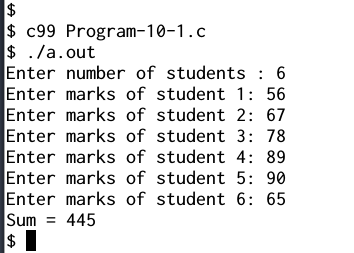
\includegraphics[scale=0.6]{Output-10-1.png}
\caption{Sum of marks}
\label{output-10-1}
\end{center}
\end{figure}

Note that if the number of students is more than 10, or if a number more than 10 is entered by mistake, the behaviour of this program is not at all good. This is one of the problem areas of C. While it is solveable, it requires lot of extra, painstaking work and is error-prone.
 
\subsection*{Multi-Dimensional Arrays}
The array which is used to represent and store data in a tabular form is called as `two dimensional array.' Such type of array specially used to represent data in a matrix form.

In C, we essentially create arrays of arrays to provide multi-dimensional arrays.

\textbf{\texttt{data\_type array\_name[rows][columns];}}

\subsubsection*{Example} 

\lstinline!float a[3][6];!

Here, a is a multi-dimensional array; specifically a two dimensional array. This has 3 rows and 6 columns.

\begin{table}[ht]
\centering
\begin{tabular}{|c|c|c|c|c|c|c|}\hline
      & col 1   & col 2   & col 3   & col 4   & col 5   & col  6\\\hline
row 1 & a[0][0] & a[0][1] & a[0][2] & a[0][3] & a[0][4] & a[0][5]\\\hline
row 2 & a[1][0] & a[1][1] & a[1][2] & a[1][3] & a[1][4] & a[1][5]\\\hline
row 3 & a[2][0] & a[2][1] & a[2][2] & a[2][3] & a[2][4] & a[2][5]\\\hline
\end{tabular}
\caption{Multi-dimensional Array::Layout}
\label{matrix}
\end{table}

\subsubsection*{Example} 
Program to find out sum of diagonal elements of the given matrix.
\lstinputlisting{Program-10-2.c}

Of course the computation loop can also be written more simply as:
\begin{lstlisting}[numbers=none]
  for (int n = 0; n < 3; n++)
       sum_diag += matrix[n][n];
\end{lstlisting}

\begin{figure}[ht]
\label{output-10-2}
\begin{center}
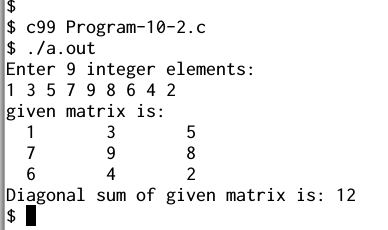
\includegraphics[scale=0.6]{Output-10-2.png}
\caption{Sum of diagonal}
\end{center}
\end{figure}

\subsection*{Things to note} 
\begin{enumerate}
\item Arrays are very useful \emph{only} when you are working with sequences of the \emph{same} kind of data. 
\item Array elements are stored in contiguous memory locations.
\item C does not have bounds checking mechanism for array sizes.
\item We cannot change size of array at the run time.
\item To delete or insert an element we need to traverse throughout the array, and copy the affected elements.
\end{enumerate}

\end{document}